% !TeX program = xelatex
% !TEX encoding = UTF-8 Unicode

\documentclass[9pt]{article}
\usepackage{hyperref}
\usepackage{ulem} 
\usepackage{mathtools}
\usepackage{enumitem}
\usepackage{color,soul}
\usepackage{inputenc}
\usepackage[margin=2.75cm]{geometry}
\usepackage{xcolor}
\usepackage{listings}

% TODO Modificare questi parametri per scrivere un bash più bello

\lstset{basicstyle=\ttfamily,
	showstringspaces=false,
	commentstyle=\color{blue},
	keywordstyle=\color{red}
}
\lstset{
	language=bash,
	basicstyle=\ttfamily
}

\begin{document}

\title{Shell Scripting 2020: Week 1}
\author{Stefan Ciprian Voinea}
\maketitle

%\begin{figure}[h!]
%	\centering
%	\includegraphics[width=12cm]{autoconfiguration.png}
%	\caption{IPv6 Autoconfiguration example}
%	\label{fig:autoconfig}
%\end{figure}

\begin{enumerate}
	\item \textbf{Directory setup}
		\begin{lstlisting}[language=bash]
mkdir ShellScripting2019
cd ShellScripting2019
mkdir Week1
cd Week1
		\end{lstlisting}

	\item \textbf{Identity shift}
		\begin{itemize}
			\item alias for \texttt{ls}:
			\begin{lstlisting}[language=bash]
alias show-files-here=ls
			\end{lstlisting}
			\item for the definition of \texttt{cman} command I wrote a simple script that opens firefox and a website that contains the manual of linux commands:
			\begin{lstlisting}[language=bash]
url='https://man.cx/'
firefox $url$1 
			\end{lstlisting}
			I set the alias with this command:
			\begin{lstlisting}[language=bash]
alias cman=./task2.sh
			\end{lstlisting}
		\end{itemize}

	\item \textbf{(NON)-logins}
	
		The \texttt{~/.bash\_aliases} file allows the system to not lose the aliases set.
		Since Ubuntu 20.04 does not have such file, I had to create it and to activate it.
		\begin{lstlisting}
touch ~/.bash_aliases
source ~/.bash_aliases
		\end{lstlisting}
		A useful alias that I can place in this file would be:
		\begin{lstlisting}
alias update='sudo -- sh -c "apt update && apt upgrade"'
		\end{lstlisting}

		\newpage
		Logging without the \texttt{bash -} command to change shell
		
		\begin{figure}[h!]
			\centering
			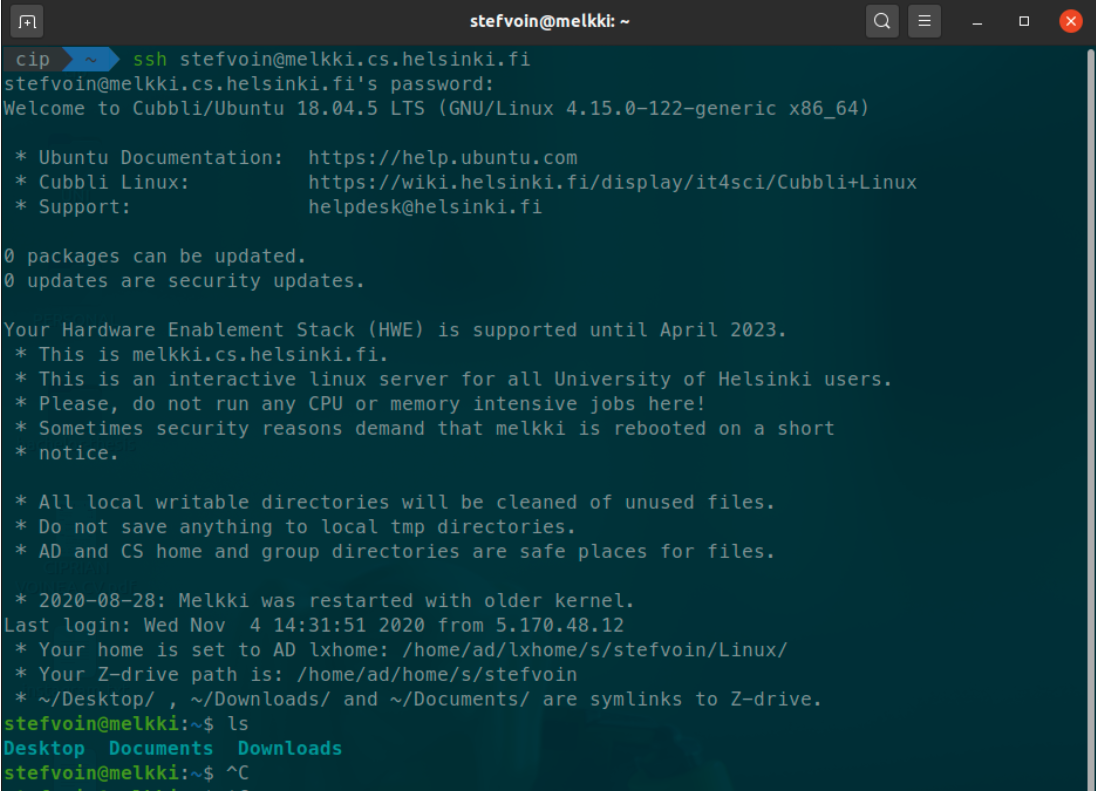
\includegraphics[width=\linewidth]{img/6_1.png}
		\end{figure}

	\item \textbf{Enter RSYNC}
		I executed these commands in \texttt{ssh}.
		\begin{lstlisting}[language=bash,breaklines=true]
# At first the directory is empty
stefvoin@melkki:~/Desktop$ ls ShellScripting2020/Week1/

# When I execute rsync without --stats there is no output, the target directory is just populated
stefvoin@melkki:~/Desktop$ rsync --archive /cs/home/tkt_cam/public_html/2018/12/01/ ShellScripting2020/Week1/
# The contents show all the files in the given folder to sync
stefvoin@melkki:~/Desktop$ ls ShellScripting2020/Week1/
201812010000.jpg  201812010300.jpg  201812010600.jpg  201812010900.jpg  201812011200.jpg  201812011500.jpg  201812011800.jpg  201812012100.jpg
201812010100.jpg  201812010400.jpg  201812010700.jpg  201812011000.jpg  201812011300.jpg  201812011600.jpg  201812011900.jpg  201812012200.jpg
201812010200.jpg  201812010500.jpg  201812010800.jpg  201812011100.jpg  201812011400.jpg  201812011700.jpg  201812012000.jpg  201812012300.jpg

# If I remove one file and execute rsync again, there will be no output, the missing file will just be restored
stefvoin@melkki:~/Desktop$ rm ShellScripting2020/Week1/201812010000.jpg 
stefvoin@melkki:~/Desktop$ rsync --archive /cs/home/tkt_cam/public_html/2018/12/01/ ShellScripting2020/Week1/

# When I execute rsync with --stats it gives me the information on the difference between the two directories
stefvoin@melkki:~/Desktop$ rsync --archive /cs/home/tkt_cam/public_html/2018/12/01/ ShellScripting2020/Week1/ --stats

Number of files: 25 (reg: 24, dir: 1)
Number of created files: 0
Number of deleted files: 0
Number of regular files transferred: 0
Total file size: 9,712,499 bytes
Total transferred file size: 0 bytes
Literal data: 0 bytes
Matched data: 0 bytes
File list size: 0
File list generation time: 0.001 seconds
File list transfer time: 0.000 seconds
Total bytes sent: 555
Total bytes received: 88

sent 555 bytes  received 88 bytes  1,286.00 bytes/sec
total size is 9,712,499  speedup is 15,104.98

# If I delete one file and then I restore it with rsync --stats, I can see that it tells me the information about the operation
stefvoin@melkki:~/Desktop$ rm ShellScripting2020/Week1/201812010000.jpg 
stefvoin@melkki:~/Desktop$ rsync --archive /cs/home/tkt_cam/public_html/2018/12/01/ ShellScripting2020/Week1/ --stats

Number of files: 25 (reg: 24, dir: 1)
Number of created files: 1 (reg: 1)
Number of deleted files: 0
Number of regular files transferred: 1
Total file size: 9,712,499 bytes
Total transferred file size: 369,426 bytes
Literal data: 369,426 bytes
Matched data: 0 bytes
File list size: 0
File list generation time: 0.005 seconds
File list transfer time: 0.000 seconds
Total bytes sent: 370,108
Total bytes received: 107

sent 370,108 bytes  received 107 bytes  740,430.00 bytes/sec
total size is 9,712,499  speedup is 26.23
		\end{lstlisting}

	\item \textbf{Time and Date}
	
		This is the command:
		\begin{lstlisting}[language=bash]
date +%A.%Y.%m.%d 
		\end{lstlisting}
		And this is the output:
		\begin{lstlisting}[language=bash]
Friday.2020.10.30
		\end{lstlisting}
		
	\item \textbf{Inserting date}
	
		The command that is contained in the file \texttt{task6.sh}:
		\begin{lstlisting}[language=bash,breaklines=true]
echo "rsync --archive /cs/home/tkt_cam/public_html/$(date +%Y/%m/%d)/~/ShellScripting2019/Week1/$(date +%A.%Y.%m.%d)"
		\end{lstlisting}
		
	\item \textbf{Two at once}
	
		By using \texttt{command >out 2>error} I can direct the \texttt{stdout} to the file \texttt{out} and the \texttt{stderr} to the file \texttt{error}.\\
		This command works, does not show any output because it is written in the \texttt{out} file.
		\begin{lstlisting}[language=bash]
ls >out 2>error
		\end{lstlisting}
		This command doesn't works because the \texttt{ghost\_directory} does not exist.
		There is no output output because it is written in the \texttt{error} file.
		\begin{lstlisting}[language=bash]
ls ghost_directoy >out 2>error
		\end{lstlisting}
		Content on error file:
		\begin{lstlisting}[language=bash]
ls: cannot access 'ghost_directory': No such file or directory
		\end{lstlisting}
		
	\item \textbf{Hey! What about STDIN?}
	
		As explained by the command \texttt{man cat}: \texttt{cat - concatenate files and print on the standard output}.
		This means that if I type \texttt{cat string}, it will print my string when I press enter, while if I type \texttt{cat filename}, it will print the contents of the file.
	
\end{enumerate}

\end{document}